\documentclass[article,12pt]{elsarticle}
\usepackage[spanish]{babel}
\usepackage[utf8]{inputenc}
\usepackage{amssymb}
\usepackage{flushend}
\usepackage{float}
\usepackage{anysize}
\usepackage{amsmath}
\usepackage{amsfonts}
\usepackage{dcolumn}
\usepackage{amsthm}
\usepackage{caption}
\usepackage{float}
\usepackage{subfigure}
\usepackage{graphicx}
\usepackage{lmodern}
\usepackage{booktabs}
\usepackage{color}
\usepackage{longtable}
\usepackage{rotating}
\usepackage{etoolbox}
\usepackage{comment}
\usepackage{pdflscape}
\usepackage{booktabs}
\usepackage{float}


\begin{document}

\begin{frontmatter}
    \title{Laboratorio de Electromagnetismo \\  Práctica  5\\ 
        Conductores Ohmicos y no Ohmicos}
    \author{Iván Bautista Alvarado$^1$ y Andrés López González$^1$} %Aquí va el nombre de los integrantes que participaron en el informe.
    \address{$^1$ Facultad de Ciencias, Universidad Nacional Autónoma de México, M\'exico CDMX.}


    \begin{abstract}
     This experimental report investigates the electrical behavior of several components, including resistors, a socket, a diode, and an LED, in relation to Ohm’s Law. Using a power source and a multimeter, we measured the voltage-current relationships for each element. Resistors demonstrated an ohmic behavior within specific current ranges, where the slope of the voltage-current graph aligned with the expected resistance values based on their color codes, and we also noticed that in our amper-range the socket is also an ohmic resistor. However, the diode and LED exhibited non-ohmic behavior, as their current-voltage relationships deviated significantly from linearity. This study confirms that while Ohm’s Law applies to certain materials under controlled conditions, other materials such as semiconductors require more complex models to accurately describe their behavior.
    \end{abstract}

    \begin{keyword}
     Ohm’s Law, resistors, semiconductors, non-ohmic behavior, voltage-current relationship.
    \end{keyword}
\end{frontmatter}

    
\section*{Resumen}
    Este informe experimental investiga el comportamiento eléctrico de varios componentes ampliamente usados en la electrónica, incluidas resistencias, un socket, un diodo y un LED, en relación con la Ley de Ohm. Utilizando una fuente de alimentación y un multímetro, medimos las relaciones de voltaje-corriente para cada elemento. Los resistores demostraron un comportamiento óhmico dentro de rangos de corriente específicos, donde la pendiente del gráfico de voltaje-corriente se alineó con los valores de resistencia esperados según sus códigos de color, y también notamos que en nuestro rango de amperios el socket también es un resistor óhmico. Sin embargo, el diodo y el LED exhibieron un comportamiento no óhmico, ya que sus relaciones de corriente-voltaje se desviaron significativamente de la linealidad. Este estudio confirma que, si bien la Ley de Ohm se aplica a ciertos materiales en condiciones controladas, otros materiales, como los semiconductores, requieren modelos más complejos para describir con precisión su comportamiento.

\noindent \textit{Palabras Clave}: Ley de Ohm, Resistencias, Semiconductores, Comportamiento no óhmico, Relación voltaje-corriente.\\ \hline

\section{Introducción}
Cuando hablamos de corrientes eléctricas, no solo debemos considerar un flujo de electrones, sino también el medio por el que está pasando esa corriente eléctrica. Esto es lo que nos dice la \textbf{Ley de Ohm}
\begin{equation}
    V=RI
\end{equation}
que se deduce experimentalmente.
Sin embargo, esta ley solo es válida para algunos materiales, a los que les llamamos materiales ohmicos. Pero existen también otro tipo de materiales que no siguen una correlación lineal entre la corriente que reciben y el voltaje que induce esa corriente. A los que llamamos materiales no Ohmicos

Para entender un poco mejor cuándo la ley de Ohm falla, debemos verla de otra manera:
\begin{equation}
    J= \sigma E
\end{equation}
En donde $\sigma$ es la conductividad del material, E es el campo eléctrico que $"$empuja$"$ a las cargas y J es la densidad de corriente $J=I/A$.
En este caso, la conductividad $\sigma$ no depende de la longitud, del volumen ni de la forma del material, únicamente depende de su estructura microscópica. Y por lo tanto, es una propiedad intrínseca del material. Al analizarlo de manera microscópica, nos damos cuenta de que $\sigma$ depende del promedio del tiempo que hay entre cada colisión que tiene una partícula cargada y otra partícula dentro del medio. Si el campo eléctrico E que mueve a las partículas cargadas no es muy intenso, ese tiempo promedio de colisión va a ser constante y no va a cambiar. Pero si el campo eléctrico es muy intenso, el tiempo promedio de colisión va a empezar a variar, y en casos extremos, las colisiones serán tan extremas que las particulas que se encontraban neutras eléctricamente pasarán a ionizarse, creando así más partículas cargadas.
Entonces notamos que la Ley de Ohm solo es válida para ciertos intervalos de campo eléctrico en donde no sea muy intenso.
Pero la propia estructura del material puede ser la causa de que no respete la Ley de Ohm, esto suele darse en materiales semiconductores.
    \subsection{Hipótesis}
    El foco Led, el diodo y la resistencia deberían presentar un comportamiento ohmico. Pero el transistor y el diodo no.
    \subsection{Objetivos}
    Ver cuáles objetos se comportan de acuerdo a la Ley de Ohm y cuáles no.
\section{Desarrollo Experimental / Métodos}
 Materiales utilizados:
    \begin{itemize}
        \item 1 Fuente de poder
        \item 1 Multímetro
        \item 4 cables banana-banana
        \item 2 Caimanes
        \item Resistencias de 100 $\Omega \sim $ 300 $\Omega$
        \item 1 Foco con socket
        \item 1 Foco Led
        \item 1 Transistor
        \item 1 Diodo
    \end{itemize} 
    El desarrollo consistió en pasar corriente eléctrica por la resistencia, el foco con socket, el foco led, el diodo y el transistor.

    Se conectó la fuente de poder al multímetro desde la fuente negativa a la entrada común del multímetro (entrada negra), para poder medir el amperaje, y la entrada roja del multímetro la conectamos, con ayuda de un caiman, a la terminal del objeto que queremos observar su comportamiento. Y del otro lado, también con ayuda de un caimán, conectamos la entrada positiva de la fuente a la otra terminal del objeto.
    El dónde conectar los cables con los caimanes en el objeto va a depender de este mismo. Como se ilustra en la figura:
    \begin{figure}[H]
    \centering
    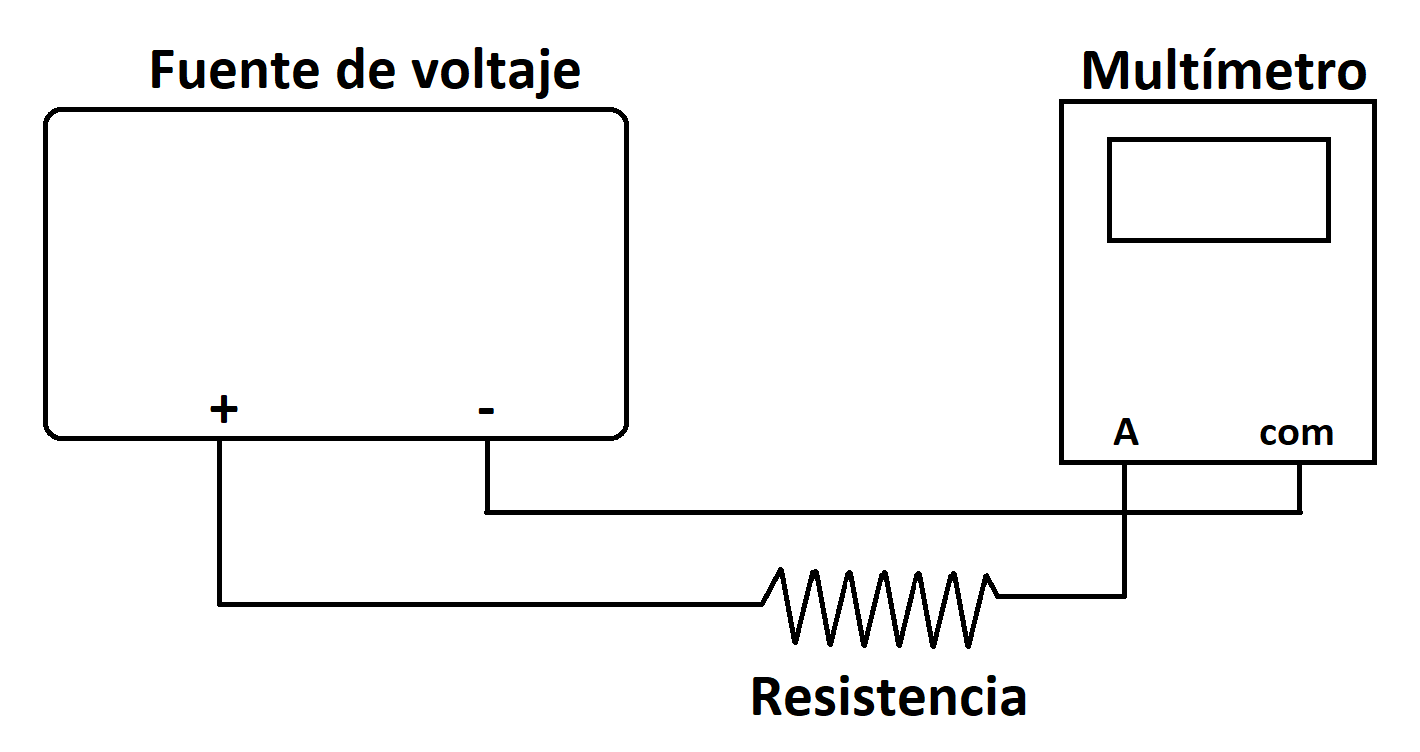
\includegraphics[width=0.6\linewidth]{Arreglo.png}
\end{figure}

    Para la resistencia es indiferente la terminal que a la que se conecten.
    Para el foco led, debemos conectar la conexión positiva al cable largo, y en el pequeño va la conexión negativa.
    Para el transistor, la terminal de la base va conectada a la conexión positiva, y el emisor va a la negativa.
\section{Resultados y discusión}
Para la primera resistencia obtuvimos la siguiente gráfica (Figure 1.).
\begin{figure}[h]
    \centering
    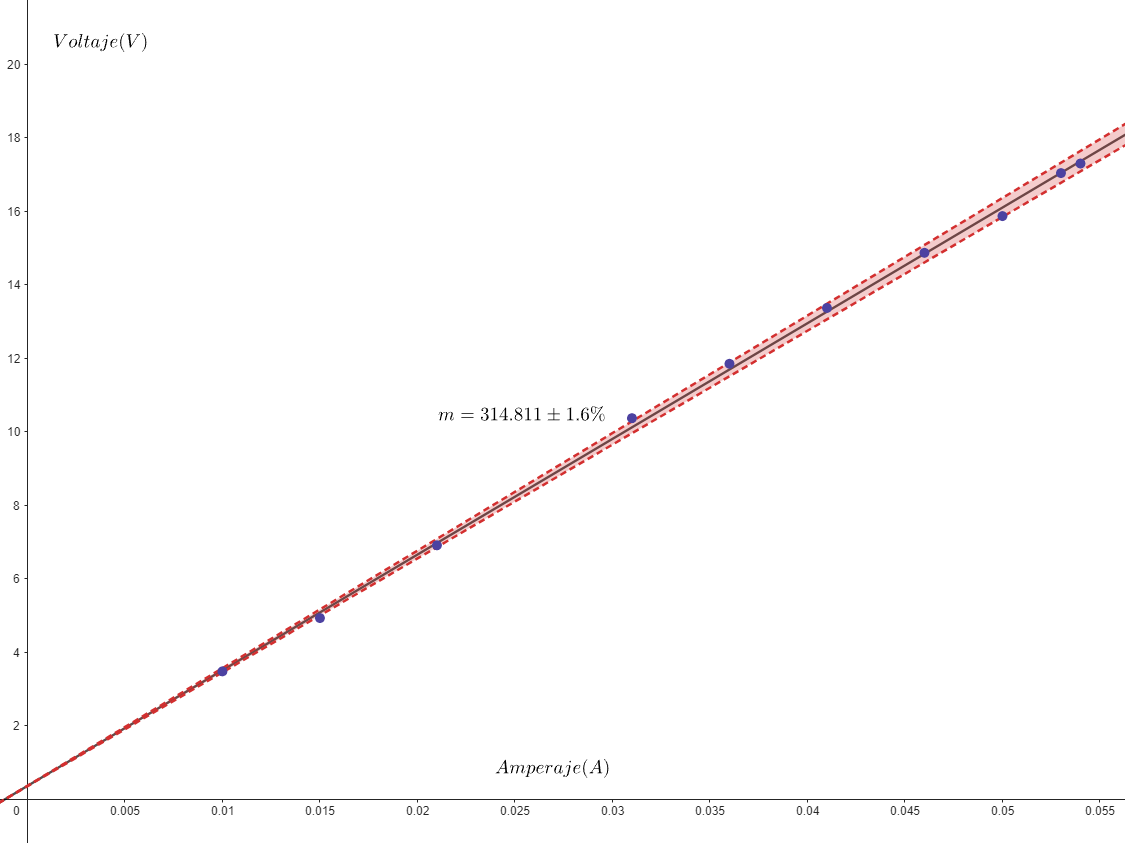
\includegraphics[width=0.8\linewidth]{resis1.png}
    \caption{Comportamiento de la primera resistencia (V vs A)}
    \label{fig:enter-label}
\end{figure}
Vease que para este gráfico (y en los siguientes), al ajustar los puntos por una regresión lineal se obtiene que su pendiente es la resistencia del objeto; en este caso obtenemos que en el intervalo de 0A a 0.054A la resistencia es de $314.811 \Omega \pm 1.6\%$, lo cual nos parece un dato muy correcto pues de acuerdo al código de colores este nos indica que su resistencia es de 300 $\Omega$, la resistencia nos parecía claro que obedezca la ley de Ohm pues es el elemento primordial cuando se habla de resistencias y ley de ohm, pero con esto hemos comprobado tanto la ley como lo que nos indicaba el código de colores. \\

Para la segunda resistencia se obtiene el siguiente gráfico.\\

\begin{figure}[H]
    \centering
    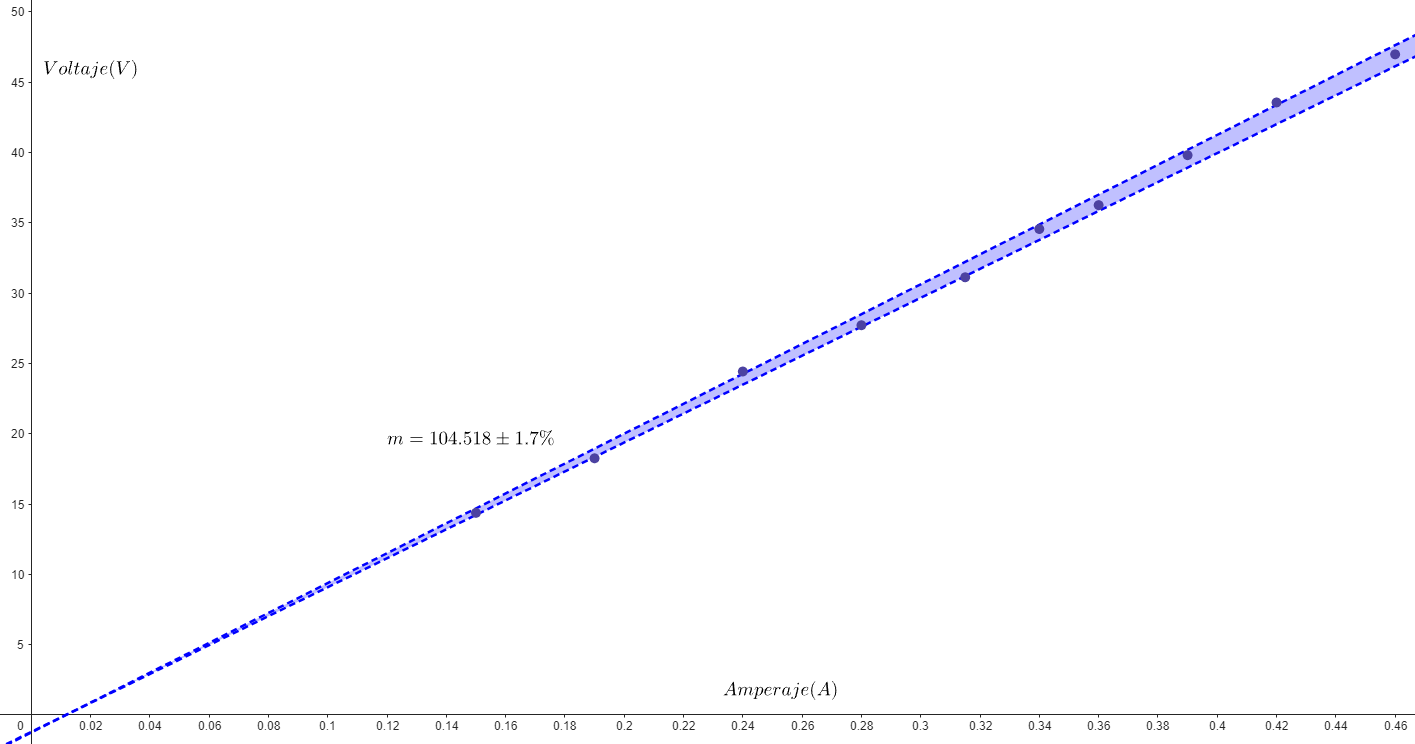
\includegraphics[width=0.8\linewidth]{resis2.png}
    \caption{Comportamiento de la segunda resistencia (V vs A)}
    \label{fig:enter-label}
\end{figure}

Para este caso nuevamente se cumple la ley de Ohm (en el intervalo de 0A a 0.46A), hemos deducido que la resistencia es de $104.518 \Omega \pm 1.7\%$, en este caso teníamos duda si el color que estábamos viendo en la primera línea era café o roja, lo que ha sido aclarado una vez visto este gráfico, es entonces que descubrimos que era café y la resistencia según su código de colores indicaba ser de 100 $\Omega$. \\

Para el socket, obtenemos el siguiente gráfico (Figure 3). Vease que cumple ley de Ohm, al menos en el intervalo en el que hemos podido evaluarlo (nuestra fuente de poder no alcanzaba mayores valores), siendo este intervalo de 0A a 3.786A. Nuestro resultado es que su resistencia es de $184.001\Omega\pm1.3\%$, sin embargo hay que poner especial atención al intervalo en el que estamos trabajando, pues según todas las bibliografías consultadas en internet el verdadero comportamiento del socket es no óhmico, solamente bajo una pequeña cantidad de amperaje se comporta como tal y hemos descubierto que esto es verdad.\\
\begin{figure}[H]
    \centering
    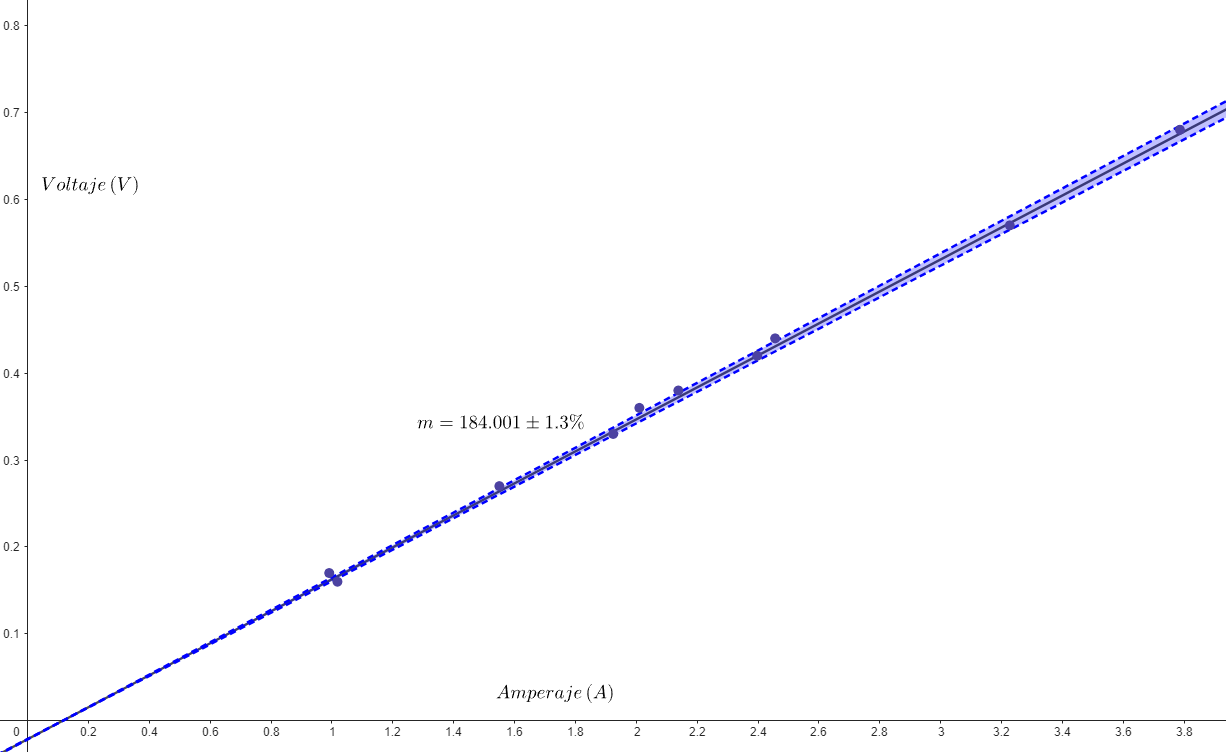
\includegraphics[width=0.7\linewidth]{sock.png}
    \caption{Comportamiento del socket (V vs A)}
    \label{fig:enter-label}
\end{figure}

Veamos el comportamiento para el diodo.\\
\begin{figure}[H]
    \centering
    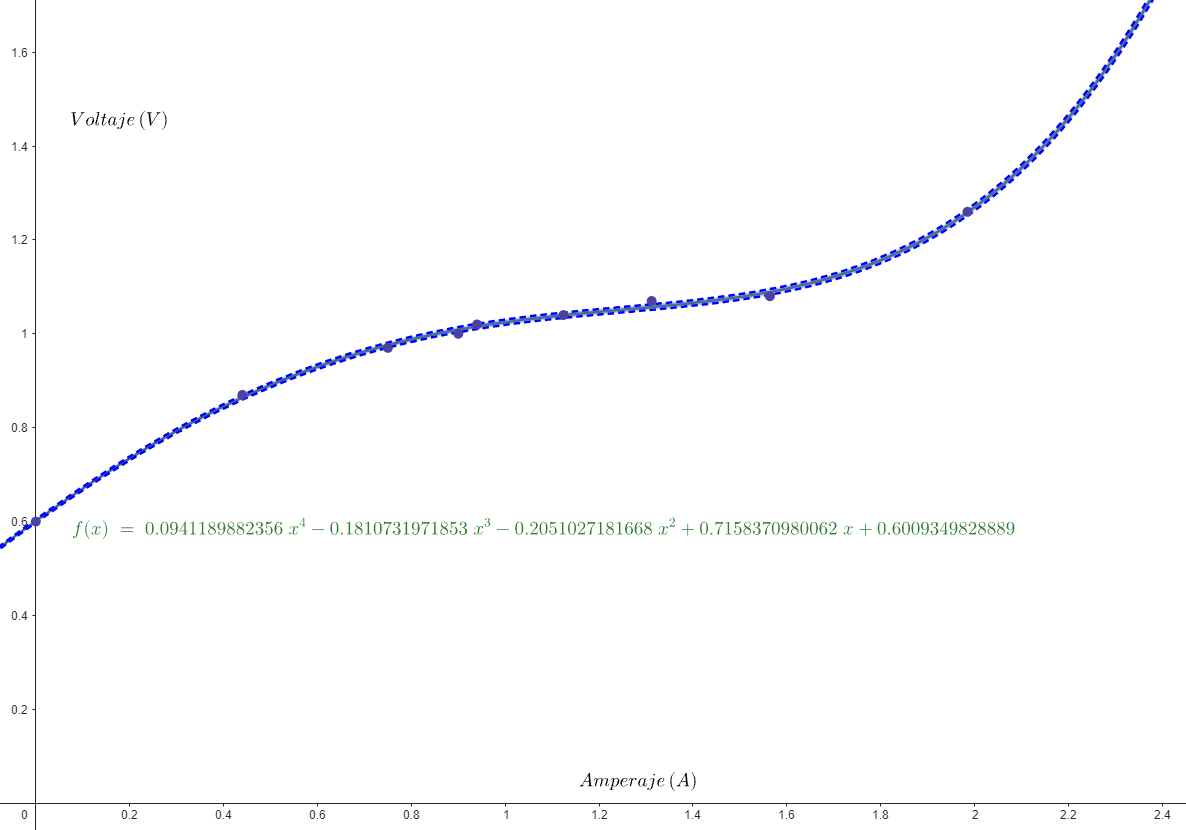
\includegraphics[width=0.75\linewidth]{diod.png}
    \caption{Comportamiento del diodo (V vs A)}
    \label{fig:enter-label}
\end{figure}
No cumple ley de Ohm, el ajuste lineal es extremadamente impreciso y solo con un polinomio de cuarto grado es posible aproximar su comportamiento pues el logarítmico presenta indeterminaciones que lo hacen imposible de sacar. En cualquier caso, este polinomio tampoco es preciso pues claramente no puede subir tan fuertemente a partir de los 2A; para este análisis se usó el intervalo de 0A a 1.985A.\\

Finalmente para el LED.\\
\begin{figure}[H]
    \centering
    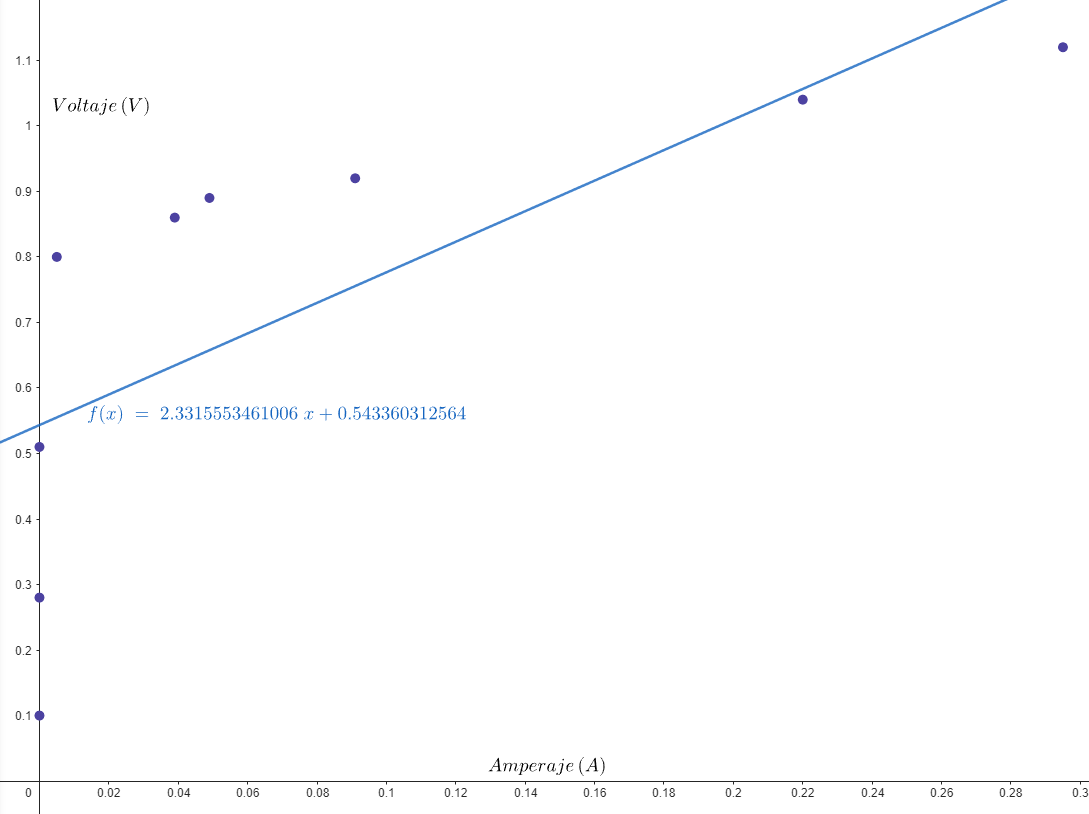
\includegraphics[width=0.75\linewidth]{led.png}
    \caption{Comportamiento del LED (V vs A)}
    \label{fig:enter-label}
\end{figure}
Este fue analizado en el intervalo de 0A a 0.295A, como se puede observar en el gráfico no sigue ley de Ohm y de hecho tampoco es posible aproximarla por un polinomio de forma que mantenga la coherencia (tampoco logarítmicamente, nuevamente, por las indeterminaciones).

\section{Conclusiones}
En este experimento, hemos explorado el comportamiento de diversos componentes electrónicos en relación con la Ley de Ohm, identificando cuáles de ellos se comportan de manera ohmica y cuáles no. Como era de esperar, las resistencias y el socket presentaron un comportamiento mayoritariamente ohmico en los intervalos de corriente que pudimos observar. Sin embargo, en el caso del socket, notamos que solo bajo un rango limitado de corriente la Ley de Ohm se mantiene, no podemos asegurarlo para rango más altos, pues la literatura sugiere un comportamiento no ohmico a mayores corrientes.\\

En el caso del diodo y el LED, confirmamos que estos no obedecen la Ley de Ohm, tal como se anticipaba. Sus gráficos mostraron relaciones no lineales entre el voltaje y la corriente. Esto es consistente con las propiedades físicas de estos dispositivos, que tienen un comportamiento altamente no lineal debido a su estructura y mecanismos de conducción.\\

Este estudio nos permite apreciar mejor las limitaciones y aplicaciones de la Ley de Ohm, destacando cómo su validez depende no solo del tipo de material, sino también de las condiciones de operación, como la intensidad del campo eléctrico y el tipo de componente. En especial, los dispositivos semiconductores presentan una complejidad adicional que no puede ser capturada por un modelo lineal simple, lo cual es crucial para el diseño y análisis de circuitos en el ámbito de la electrónica moderna.\\

\newpage
\noindent {\bf Declaración de contribución de los autores}\\ 

Iván Bautista Alvarado$^1$ y Andrés López González$^1$ hemos realizado tanto el apartado escrito como el análisis de manera colectiva siendo una participación del 100\% por parte de ambos y no solo una repartición.\\ 

{\bf Agradecimientos} \\ 

A ese.\\

\begin{figure}[h]
    \centering
    
\includegraphics[width=0.5\linewidth]{el.png}
    \caption{Electrogato}
    \label{fig:enter-label}
\end{figure}\\

\begin{thebibliography}{99}

\bibitem{griffiths}
D. J. Griffiths, \textit{Introduction to Electrodynamics}, 3rd ed. Upper Saddle River, NJ, USA: Prentice-Hall, 1999.

\bibitem{jackson}
J. D. Jackson, \textit{Classical Electrodynamics}, 3rd ed. New York, NY, USA: Wiley, 1998.

\bibitem{sadiku}
M. N. O. Sadiku, \textit{Elements of Electromagnetics}, 6th ed. New York, NY, USA: Oxford University Press, 2014.

\bibitem{wangsness}
R. K. Wangsness, \textit{Electromagnetic Fields}, 2nd ed. New York, NY, USA: Wiley, 1986.

\bibitem{zangwill}
A. Zangwill, \textit{Modern Electrodynamics}. Cambridge, UK: Cambridge University Press, 2013.

\bibitem{purcell}
E. M. Purcell and D. J. Morin, \textit{Electricity and Magnetism}, 3rd ed. Cambridge, UK: Cambridge University Press, 2013.

\bibitem{shadowitz}
A. Shadowitz, \textit{The Electromagnetic Field}. Mineola, NY, USA: Dover Publications, 1988.


\end{thebibliography}


\end{document}